\documentclass[conference,10pt,compsocconf]{IEEEtran}

% *** CITATION PACKAGES ***
%
\usepackage{cite}
% cite.sty was written by Donald Arseneau
% V1.6 and later of IEEEtran pre-defines the format of the cite.sty package
% \cite{} output to follow that of IEEE. Loading the cite package will
% result in citation numbers being automatically sorted and properly
% "compressed/ranged". e.g., [1], [9], [2], [7], [5], [6] without using
% cite.sty will become [1], [2], [5]--[7], [9] using cite.sty. cite.sty's
% \cite will automatically add leading space, if needed. Use cite.sty's
% noadjust option (cite.sty V3.8 and later) if you want to turn this off.
% cite.sty is already installed on most LaTeX systems. Be sure and use
% version 4.0 (2003-05-27) and later if using hyperref.sty. cite.sty does
% not currently provide for hyperlinked citations.
% The latest version can be obtained at:
% http://www.ctan.org/tex-archive/macros/latex/contrib/cite/
% The documentation is contained in the cite.sty file itself.
%
\usepackage{setspace}
\usepackage{wrapfig}
\usepackage[usenames, dvipsnames]{color}
\usepackage{balance}
\usepackage{mathtools}
\usepackage{multirow}

%\usepackage[pdftex]{graphicx}
\usepackage{graphicx}
% declare the path(s) where your graphic files are
\graphicspath{{./}{./figs}}
% and their extensions so you won't have to specify these with
% every instance of \includegraphics
\DeclareGraphicsExtensions{.pdf,.jpeg,.png}

% *** SUBFIGURE PACKAGES ***
\usepackage[tight,footnotesize]{subfigure}
% \usepackage{subfigure}
% subfigure.sty was written by Steven Douglas Cochran. This package makes it
% easy to put subfigures in your figures. e.g., "Figure 1a and 1b". For IEEE
% work, it is a good idea to load it with the tight package option to reduce
% the amount of white space around the subfigures. subfigure.sty is already
% installed on most LaTeX systems. The latest version and documentation can
% be obtained at:
% http://www.ctan.org/tex-archive/obsolete/macros/latex/contrib/subfigure/
% subfigure.sty has been superceeded by subfig.sty.

%\usepackage[caption=false]{caption}
%\usepackage[font=footnotesize]{subfig}
% subfig.sty, also written by Steven Douglas Cochran, is the modern
% replacement for subfigure.sty. However, subfig.sty requires and
% automatically loads Axel Sommerfeldt's caption.sty which will override
% IEEEtran.cls handling of captions and this will result in nonIEEE style
% figure/table captions. To prevent this problem, be sure and preload
% caption.sty with its "caption=false" package option. This is will preserve
% IEEEtran.cls handing of captions. Version 1.3 (2005/06/28) and later
% (recommended due to many improvements over 1.2) of subfig.sty supports
% the caption=false option directly:
%\usepackage[caption=false,font=footnotesize]{subfig}
%
% The latest version and documentation can be obtained at:
% http://www.ctan.org/tex-archive/macros/latex/contrib/subfig/
% The latest version and documentation of caption.sty can be obtained at:
% http://www.ctan.org/tex-archive/macros/latex/contrib/caption/

% *** PDF, URL AND HYPERLINK PACKAGES ***
%
\usepackage{url}
% url.sty was written by Donald Arseneau. It provides better support for
% handling and breaking URLs. url.sty is already installed on most LaTeX
% systems. The latest version can be obtained at:
% http://www.ctan.org/tex-archive/macros/latex/contrib/misc/
% Read the url.sty source comments for usage information. Basically,
% \url{my_url_here}.

% *** Do not adjust lengths that control margins, column widths, etc. ***
% *** Do not use packages that alter fonts (such as pslatex).         ***
% There should be no need to do such things with IEEEtran.cls V1.6 and later.
% (Unless specifically asked to do so by the journal or conference you plan
% to submit to, of course. )

\usepackage{draftwatermark}

\newcommand{\assign}[1]{\textcolor{red}{(#1)}}
\newcommand{\todo}[1]{\textcolor{Orange}{TODO: #1}}
\newcommand{\fixme}[1]{\textcolor{green}{(#1)}}

\begin{document}
\title{Towards Total Knowledge of I/O through Integrated Multicomponent Instrumentation}

\maketitle

\begin{abstract}
%%% I had to submit a 150-word abstract to SC, so below is the shortened
%%% version I submitted
%
% As scientific computing becomes more data-intensive and storage hierarchies
% deepen, I/O performance is becoming increasingly critical to productivity in
% HPC.  Instrumentation and analysis tools have long been used to understand
% parallel I/O performance, but analyzing the individual components of I/O
% subsystems in isolation fails to answer how these components interact and
% result in poor I/O performance.
%
% To this end, we have developed a framework for holistic I/O characterization
% that integrates instrumentation from file system servers, applications, file
% system health monitors, and other system resources.  Along with formalized
% periodic regression benchmarking, we then demonstrate this framework's
% portability and unobtrusiveness by deploying it in production on two
% leadership-class computing platforms.  Using data collected during a month
% long study, we provide unique insights into applications' I/O performance
% that are enabled by this approach.  We then extend these findings to provide
% a broader understanding of how application performance varies across
% different file systems and workloads.

I/O efficiency is essential to productivity in scientific computing,
especially as most scientific domains become more data-intensive and
new large-scale computing platforms incorporate more complex storage
hierarchies.  A variety of instrumentation and analysis tools have been
utilized to great effect to help understand and optimize specific aspects of
HPC I/O, such as application access patterns, storage device traffic, and
distributed file system configurations.  However, analyzing individual services in the
I/O ecosystem in isolation fails to provide insight into the most important
questions: how do the I/O components interact, what \emph{combinations}
of optimizations across the stack are most effective, and what are the
underlying causes and effects of I/O performance problems?

In this work we explore the potential for holistic I/O characterization
by combining I/O instrumentation data from multiple sources to obtain
insights that were previously unobtainable. We describe a methodology that
incorporates file system instrumentation, application instrumentation,
health monitoring, and formalized periodic regression benchmarking and demonstrate
the applicability, portability, and unobtrusiveness of this approach by
deploying it in production on two distinct leadership-class computing
platforms.
%
% Based on our month-long study, we demonstrate the utility of our
% methodology through case studies that highlight how holistic I/O
% characterization can improve our understanding of scientific applications'
% I/O performance. We then extend these findings to provide broader insights
% into how parallel file systems perform under different types of load.
%
% PHC: I don't think this is going to be a month-long study, right? Tuning
% text here a little accordingly
%
We apply our holistic I/O characterization methodology to case studies
that highlight how it can be used to improve our understanding of
scientific application performance.  We also extend these findings to
provide broader insights into how parallel file systems perform under
different types of load.

\end{abstract}

\section{Introduction} \label{sec:introduction}

% \emph{From Rob}: I think a component of the story is that when we approach
% these problems, there are a few challenges:
% \begin{enumerate}

% \item increasing number of interoperating components (in this case, additional
% BB and DVS and so forth)

The stratification performance and capacity in storage technology is 
motivating the design of increasingly complex parallel storage systems architectures.  For
example, leadership-class computing systems are now being deployed with
flash-based, on-fabric burst buffer tiers~\cite{Henseler2016} that provide even higher performance
than traditional disk-based scratch file systems~\cite{Bhimji2016}.  Although designed to provide optimal performance and
capacity on an economic basis, this increasing number of interoperating
components also complicates the task of understanding I/O performance.

% \item different components have different "views" on I/O, different levels of
% monitoring, some of which aren't practical in production

The current state of practice is to monitor each component in the I/O stack
separately.  However, different components approach I/O from different
perspectives, often resulting in component-level monitoring data that are not
obviously compatible.  For example, server-side monitoring tools such as
LMT\cite{lmt} measure a limited number of metrics as a high-frequency time
series to achieve
low overhead, while application-level profiling tools such as
Darshan\cite{carns200924} track metrics that are expressed as bounded
summaries of individual jobs.
Data types representing the same logical
quantity, such as data written, may also be expressed in different units such
as bytes, pages, and blocks.  Bytes written at one level may also be
transformed by aggregation, coalescing, and caching before reaching another
level.

% \item no current framework for integration, lots of expert knowledge to
% construct the story of what happened and how to fix.

At present, the gaps of information resulting from these incompatibilities are
filled using expert knowledge.  Because this is
neither a scalable nor sustainable model for diagnosing performance variation in
the larger, more complicated I/O subsystems being deployed, there exists a need
for a framework that integrates data from across all components and presents a
coherent, holistic view of the inter-dependent behavior of these components.  To
this end, we have developed a framework for holistic instrumentation of I/O
subsystems known as the Total Knowledge of I/O (TOKIO) framework.  TOKIO
combines server-side and application-level performance data to
provide deeper insight into the factors that affect I/O performance in a way
that is generalizable to different architectures.

One of the most fundamental challenges in understanding I/O performance
is is how to gauge the performance and behavior of application within a
broader context absent the application of expert institutional knowledge.
Does the I/O performance of a given job meet expectations given the
capabilities of the system and the nature of the access pattern?
To this end, one of the initial goals of TOKIO is to differentiate
general performance expectations (\emph{I/O climate}) from transient
effects (\emph{I/O weather}).  The I/O climate is determined by the
characteristics of storage components, their age and capacity, and the
way they generally respond to a specific workload.  The I/O weather is
determined by momentary job scheduler load, contention, and short-term
failure events.  Through a universal metrics and measurements interface
(TOKIO-UMAMI), we demonstrate how a job's I/O performance can be quickly
classified as being within the expected variation of the file system
climate, or if it can be attributed to an extreme file system weather
event.

% \end{enumerate}

The primary contributions of this work are as follows:

\begin{itemize}
\item A proposed model for holistic instrumentation of I/O subsystems,
including identification of the key roles that individual data streams play
\item An implementation of this model on two large-scale, diverse HPC
platforms
\item A demonstration of the types of insights that can be gleaned from this
approach based on a case study of N scientific applications executed in a
production environment
\end{itemize}

In section \ref{sec:methods} and \ref{sec:platforms} we describe the tools, tests, and
platforms used to conduct this work.  In sections \ref{sec:results/overview} we summarize the
statistical features of the benchmark results and highlight interesting features
that arise from combining the application-level Darshan logs with server-side
file system logs.  In section \ref{sec:results/discussion} we then explain \emph{why} the
features described in section \ref{sec:results} arose by correlating and
comparing different data sources and including information from our own
understanding of the Lustre and GPFS architectures.  We then go on to make
broader conclusions about general parallel I/O behavior we observed at both
ALCF and NERSC, and make risky assertions about GPFS and Lustre based on those
observations that were consistently true at one site but not the other.

\section{Instrumentation methods} \label{sec:methods}

We identified the following categories of ongoing instrumentation as being
critical to understanding both the I/O climate and I/O weather of a
production system.  \todo{overview diagram here?}

\subsection{Application behavior}
\label{sec:methods/darshan}

Application behavior refers to the I/O pattern of a job as expressed from
the perspective of the application itself (i.e., the I/O pattern of the
application itself before any system-level optimizations are applied).
We rely on the Darshan I/O characterization tool~\cite{TODO}
to capture this information.  Darshan transparently records concise,
bounded statistics about an application, such as the amount of time it
spent performing I/O, the distribution of access sizes, and what files
were accessed.  Reduction, compression, and storage of these statistics
is deferred until the application exits in order to minimize overhead.
Darshan has two notable properties that are desirable for use in TOKIO.
Because of it's lightweight design, Darshan can be deployed for all
production applications on large-scale systems without perturbing
performance.  Because it operates at the application level, it is also highly
portable and can be deployed on nearly any major HPC platform.

% PHC: does the modularity thing have an impact on the rest of the paper?
%
% Recently, Darshan's architecture has been modularized to allow new sources
% of I/O data to be more easily integrated into its summaries \cite{snyder2016modular}.
% This modification allows for data from distinct components within the deep
% HPC I/O stack to be more easily correlated, providing a more comprehensive view
% of application I/O behavior. For instance, data captured from higher-level I/O
% libraries like HDF5 and MPI-IO can be correlated with data from the POSIX layer
% to determine potential inefficiencies in an I/O workload. Also, this modularized
% version of Darshan includes a Lustre module that can be correlated with data from
% other modules to gain insight into how an I/O workload interacts with the
% underlying file system.

\subsection{Storage system traffic}

Storage system traffic refers to the aggregate system-wide I/O workload
observed by the primary storage system.  On most modern-day HPC systems this
is is reflected in the aggregate traffic that reaches the parallel file
system, and is most easily represented with ongoing time-series metrics.

\label{sec:methods/lmt}
The most widely used tool for this purpose on Lustre file systems is the Lustre
Monitoring Tool (LMT).  LMT collects Lustre-specific
counters from \texttt{/proc/fs/lustre} on each Lustre OSS and MDS and presents
them to external consumers via a MySQL database.  NERSC Edison implements LMT
as a part of the Cray Sonexion Lustre platform \cite{Keopp2014}, and we built
upon the pyLMT framework developed at NERSC \cite{Uselton2009} to preserve
server-side metrics during benchmark runs across all file systems evaluated.
These metrics include bytes read and written, CPU load averages, and metadata
operation rates on a per-server basis at five-second intervals.

\label{sec:methods/ggiostat}
We developed the \emph{ggiostat} tool in order to collect analogous data from
IBM Spectrum Scale (GPFS) file systems.  \assign{Zach}  It relies upon the
\texttt{mmpmon} monitoring system in GPFS to retrieve metrics from server and
client clusters.  These metrics are queried on five second intervals by a
persistent monitoring daemon and stored in an IBM DB2 database.
The metrics collected include bytes read and written,
read and write operations, and number of inode updates \todo{(is this
a proxy for metadata operation rates?)}.

\subsection{Health monitoring \assign{Glenn and Kevin}}
\label{sec:methods/health}

Health monitoring refers to the current fault status and capacity of the
storage system: what components are offline, and how much storage space
remains on the available components.

For Lustre we do \todo{something}, and for GPFS we do \todo{something
else.}

\subsection{Job scheduling \assign{Glenn and Kevin}}

Job scheduling refers to the mix of concurrent application jobs that are
running on the compute resources of a system at any given time.
\todo{describe how we pull concurrent job activity from Edison and Mira?}

\subsection{I/O performance regression tests}

Passive monitoring and logging are critical for TOKIO, but they have a
notable shortcoming in that they don't necessarily observe any controlled
reference point: the workload and state of the system evolves over time.  In
order to compensate for this, we also incorporate routine I/O performance
regression tests as a key element of our framework.
\todo{is this what we are refering to as TOKIO-ABC?  Define?}  I/O
performance is not well-represented by a single benchmark result, however;
each storage system has its own strengths and weaknesses for different
workloads.  We therefore subdivide our regression testing into a suite of
representative applications:

\begin{itemize}
\item \textbf{HACC} \assign{Shane}
\item \textbf{VPIC} \assign{Suren} 
Vector particle-in-cell (VPIC) is a highly scalable code developed to simulate
interactions among trillions of plasma physics particles  \cite{Bowers2008}.
VPIC-IO kernel extracts the I/O operations of a magnetic reconnection
simulation, where each MPI process writes 8M (i.e., 8*1024*1024) particles. Each
particle has eight properties (six floating point and two integer) and each
property is a single dimension array. The total number of particles depend on
the number of MPI ranks used. The kernel uses H5Part API \cite{H5Part} to write
the data to a single shared HDF5 file. The execution of the kernel includes
creating and opening a file, writing data to the file, and closing the file.

\item \textbf{BDCATS} \assign{Suren} The BD-CATS-IO benchmark emulates the I/O
pattern of the BD-CATS clustering system~\cite{Patwary2015}, and it represents
one of the analyses that is performed on the output of VPIC's particle data files.
For this study, we emulate the I/O workload of a clustering both particle
positions and momenta in three dimensions.  This amounts to 75\% of the data
contained in the HDF5 file (generated by the VPIC-IO kernel) being read.

\item \textbf{IOR} \assign{Shane} The IOR benchmark has been used extensively
to characterize the performance characteristics of parallel file systems\cite{Yildiz2016,Xie2012,Lofstead2010,Uselton2010}
due to its extensive configurability.  For the purposes of this work, we applied
IOR to determine each file system's performance variability under conditions
where an application is performing I/O using the ideal parameters for each
file system.

\end{itemize}

This benchmark suite is encapsulated in a single meta-job that is executed
daily in order to provide a controlled referency point for I/O behavior on
the system.  We scale the size of this meta-job according to the
characteristics of the system on which TOKIO is deployed.  Our two goals in
selecting the size are a) to attempt to saturate the storage system and b) to
choose a job size that can realistically matriculate through the scheduler on
a daily basis within the system's normal workload mix.

\section{Data integration}

\todo{PHC: fill this in.  Maybe it comes after experimental platforms?  At
any rate, say something, even if brief, about how we bring together all of
the instrumentation sources we listed into a coherent data set.}

\section{Experimental platforms} \label{sec:platforms}

We have deployed the TOKIO framework on two distinct platforms in this study.

\begin{itemize}
\item \textbf{Cori} \assign{Glenn}
\item \textbf{Mira} \assign{Phil}
\end{itemize}

\todo{Here or in evaluation, describe how we sized the jobs for each
platform.  See mailing list discussion Jan27-Feb6.  Mira has fixed ratio of
ions to compute nodes, Cori does not, leads to different characteristics.  In
either case goal is to exercise file system as much as we can within job
sizes that will get through queue in daily cadence.}  The specific details are
described in Table \ref{tab:bench-config}.

% abandon all hope ye who try to edit this stupid table by hand.  I used
% http://www.tablesgenerator.com to make it.
\begin{table*}[h]
\centering
\begin{tabular}{|c|c|c|c|c|c|c|c|}
\hline
\multirow{2}{*}{\textbf{Benchmark}}                    & \multirow{2}{*}{\textbf{I/O Motif}}                           & \multicolumn{3}{c|}{\textbf{Mira}}                        & \multicolumn{3}{c|}{\textbf{Edison}}                      \\ \cline{3-8} 
                                                       &                                                               & \textbf{\# Nodes} & \textbf{\# Procs} & \textbf{\# Bytes} & \textbf{\# Nodes} & \textbf{\# Procs} & \textbf{\# Bytes} \\ \hline
IOR                                                    & \begin{tabular}[c]{@{}c@{}}MPI-IO\\ shared file\end{tabular}  & 1,024             & 16,384            & 1.0 TiB           & 128               & 2,048             & 0.5 TiB           \\ \hline
IOR                                                    & \begin{tabular}[c]{@{}c@{}}POSIX\\ file per proc\end{tabular} & 1,024             & 16,384            & 1.0 TiB           & 128               & 2,048             & 2.0 TiB           \\ \hline
HACC                                                   & \begin{tabular}[c]{@{}c@{}}GLEAN\\ file per proc\end{tabular} & 1,024             & 16,384            & 1.5 TiB           & 128               & 2,048             & 2.0 TiB           \\ \hline
\begin{tabular}[c]{@{}c@{}}VPIC\\ BD-CATS\end{tabular} & \begin{tabular}[c]{@{}c@{}}HDF5\\ shared file\end{tabular}    & 1,024             & 16,384            & 1.0 TiB           & 128               & 2,048             & 2.0 TiB           \\ \hline
\end{tabular}
\caption{Formalized regression testing parameters}
\label{tab:bench-config}
\end{table*}

\subsection{Mira benchmark configuration} \label{sec:platforms/mirabenchmarks}

Mira's I/O architecture is fundamentally different from that of the Cray
systems at NERSC, with fixed-size partitions of compute nodes connected to
a single I/O node that forwards application I/O requests to the SAN.
Saturating the I/O bandwidth of the underlying storage servers requires the
use of many I/O nodes, meaning that peak storage bandwidth can only be
attained using a large portion of the system's available compute nodes.
Running daily I/O benchmarks that span a large portion of Mira's compute
nodes is impractical due to the lengthy queue times of capability jobs and
the obvious objection system administrators would have to this practice.

For these reasons, we decided to use 1,024 Mira compute nodes (i.e., a single
rack), a partition size that should be small enough to move quickly through
scheduler queues, but large enough to exercise an adequate portion of the
storage system. We use 16 processes per node, resulting in a total of 16,384
processes executing each benchmark. The benchmark workloads were configured
to use enough I/O volume to drive the storage system for 1--2 minutes.
Full benchmark configurations for Mira are given below in
Table~\ref{tab:bench-config}.

\section{Results} \label{sec:results}

%%%%%%%%%%%%%%%%%%%%%%%%%%%%%%%%%%%%%%%%%%%%%%%%%%%%%%%%%%%%%%%%%%%%%%%%%%%%%%%%
\subsection{Statistical Overview} \label{sec:results/overview}
%%%%%%%%%%%%%%%%%%%%%%%%%%%%%%%%%%%%%%%%%%%%%%%%%%%%%%%%%%%%%%%%%%%%%%%%%%%%%%%%

Figure \ref{fig:perf-summary-boxplots-fs} provides an overall distribution of
performance measured by all benchmarks normalized to the highest performance observed on each file system.  Mira's distribution of variation is the most narrow, with all benchmarks' 25th percentiles well above 50\% of that file system's peak performance.  By comparison, shared-file I/O performance (BD-CATS, IOR/shared, and VPIC) on Edison's file systems (scratch1-scratch3) is appreciably lower than the maximum observed peak, which correspond to file-per-process read workloads (HACC and IOR/fpp).  Although the source of this disparity in variation between Mira and Edison is not clear from \ref{fig:perf-summary-boxplots-fs} alone, we explore the underlying causes in subsequent sections.

\begin{figure}[t]
	\centering
	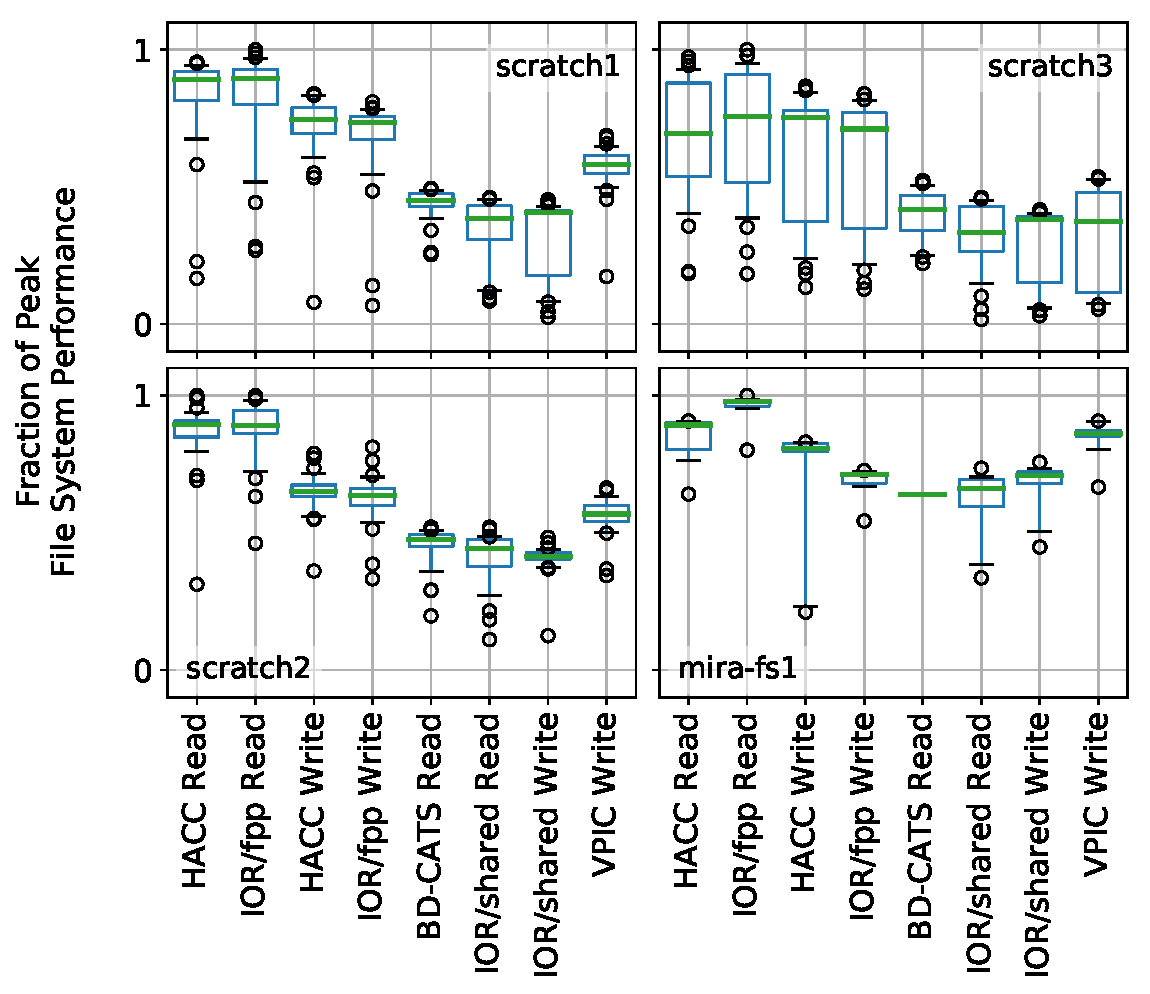
\includegraphics[width=1.0\columnwidth]{figs/perf-boxplots-per-fs.pdf}
	\caption{TOKIO-ABC I/O performance for Edison (\texttt{scratch1},
	\texttt{scratch2}, \texttt{scratch3}) and Mira (\texttt{mira-fs1}) normalized to
	the mean of all tests performed on each file system.  Each box reflects the
	distribution of all four application workloads and both read and write
	performance. Whiskers represent the 5th and 95th percentiles.}
	\label{fig:perf-summary-boxplots-fs}
\end{figure}

Such variation in peak file system performance caused by suboptimal I/O access patterns is well documented\cite{Lofstead2010,Uselton2010,Xie2012}.  To focus solely on the variation caused by factors \emph{extrinsic} to each application, we then define the \emph{fraction of peak performance} as the performance of a job divided by the maximum performance observed for all jobs \emph{of the same I/O motif} as listed in Table \ref{tab:bench-config} and whether the job did reads or writes.  For example, the fraction peak performance for a HACC write test is only normalized to the maximum performance of all other HACC write tests.  References to fraction peak performance are hereafter defined this way.

This fraction peak performance distribution, shown in Figure \ref{fig:perf-summary-boxplots-motif}, reveals that the degree of performance variation \emph{within} each application also varies with each file system.  For example, the HACC write workload is susceptible to a long tail of performance degradation on mira-fs1 despite
that file system's overall lower variation shown in \ref{fig:perf-summary-boxplots-fs}.  Similarly, all Edison file systems show a long tail of performance loss for the IOR/shared file read workload.  Edison's scratch3 also demonstrates very broad performance variation for the VPIC write workload, contrasting with the relatively narrow performance variation of this application VPIC on all other file systems.

\begin{figure}[t]
	\centering
	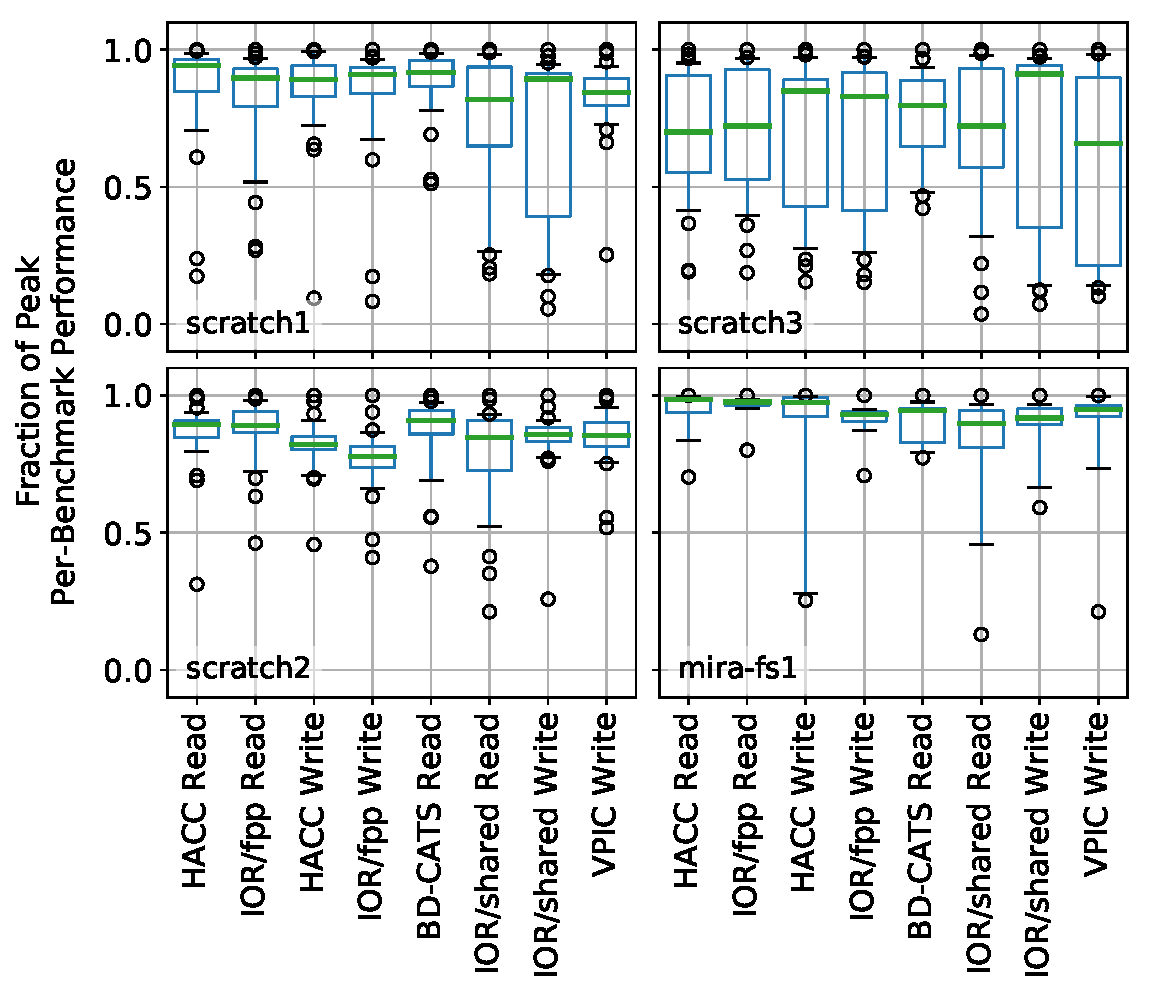
\includegraphics[width=1.0\columnwidth]{figs/perf-boxplots.pdf}
	\caption{TOKIO-ABC I/O performance for all file systems tested grouped by test
	applications and read/write mode.  Whiskers represent the 5th and 95th
	percentiles.}
	\label{fig:perf-summary-boxplots-motif}
\end{figure}

\textbf{Thus, Figure \ref{fig:perf-summary-boxplots-motif} demonstrates that the
performance variability results from factors intrinsic to the application (e.g., I/O motif) \emph{and} factors intrinsic to the file system}, and
different I/O motifs result in different levels of performance \emph{and} variability.  Furthermore, these behaviors are not a function of the parallel file system software architecture either; all Edison file systems are Lustre-based, and yet there is a marked difference in variability between scratch1/scratch and scratch3 shown in Figure~\ref{fig:perf-summary-boxplots-motif}.  Thus, these differences in performance variation must be a result of their different hardware configurations (discussed in Section \ref{sec:platforms}), their specific user workloads, or a combination of both.

%%%%%%%%%%%%%%%%%%%%%%%%%%%%%%%%%%%%%%%%%%%%%%%%%%%%%%%%%%%%%%%%%%%%%%%%%%%%%%%%
\subsection{Combining Application and Server-side Telemetry} \label{sec:results/combining}
%%%%%%%%%%%%%%%%%%%%%%%%%%%%%%%%%%%%%%%%%%%%%%%%%%%%%%%%%%%%%%%%%%%%%%%%%%%%%%%%

To obtain a better understanding of how performance variation is caused by factors extrinsic to the application, we then combine what we know from application-level analysis provided by Darshan with file system-level analysis provided by LMT (on Edison) and ggiostat (on Mira).  An intuitive source of performance loss would be from other jobs that are also consuming file system bandwidth, so to explore the effects of competing I/O traffic, we define the \emph{coverage factor} ($\mathit{CF}$) of a job $j$:

\begin{equation} \label{eq:cf}
	\mathit{CF}(j) = \frac{N_{\textup{bytes}}^{\textup{Darshan}}(j)}
	{\sum_{t,s}^{\textup{time,servers}}
	\left [ N_{\textup{bytes}}^{\textup{LMT,ggiostat}}(t,s) \right ] }
\end{equation}
%
where $N_{\textup{bytes}}^{\textup{Darshan}}$ is the number of bytes read and written by job $j$ according to its Darshan log, and $N_{\textup{bytes}}^{\textup{LMT,ggiostat}}$ is the number of bytes read and written to a parallel file system server $s$ during a 5-second time interval $t$.  The time interval over which the job ran ($\mathit{time}$) and the servers to which the job wrote ($\mathit{servers}$) are both taken from the job's Darshan log~\cite{snyder2016modular}.

The coverage factor is a direct reflection of how much I/O traffic a job
competed against in the underlying file systems.  $CF = 1.0$ when
all of the server-side I/O was caused by job $j$, while $CF = 0.5$ indicates that only half of the server-side I/O was attributable to job $j$ while the other half came from other sources.  In practice, it is possible to observe $CF > 1.0$ 
if (1) server-side monitoring (e.g., LMT or ggiostat)
did not capture data from all servers during a polling interval, or (2) clock skew exists between the compute nodes and the file system servers, causing the Darshan log and LMT/ggiostat to have an inconsistent understanding of when I/O happened.  To eliminate the most erroneous data, we discard all test results where $CF > 1.2$ in the subsequent analysis.

The distribution of coverage factors across all experiments run are shown in
Figure~\ref{fig:cdfs}a which reveals that the majority of tests
($> 85\%$ on Edison and $> 75\%$ on Mira) have high coverage factor
($CF > 0.90$).  This is consistent with the observation that I/O occurs in
bursts~\cite{Carns2011,Liu2016}, and the probability of two bursts coinciding
and causing contention for bandwidth (thereby reducing $CF$) is relatively low.  In particular, Mira's CF distribution is so narrow that over 50\% of tests effectively ran completely uncontended for bandwidth; $\textit{CF} >= 0.99$ corresponds to the 43rd percentile on that system.

Despite this low incidence of overlapping bursts, though, the cumulative
distribution function (CDF) of performance relative to the peak observed
bandwidth for each application (Figure~\ref{fig:cdfs}b) is far more broadly distributed.
Between 19\%-23\% (scratch1/scratch2) and 47\% (scratch3) of jobs on Edison got less than half of the peak observed performance, clearly indicating that the coverage factor (and therefore server-side
I/O bandwidth) is not the only contributor to sub-optimal performance.  
This finding is consistent with
the work of Uselton and Wright\cite{Uselton2013} who demonstrated that Lustre
file system performance is constrained by both the weighted sum of both bandwidth
\emph{and} I/O operation (IOP) rate.  

\begin{figure}[t]
	\centering
	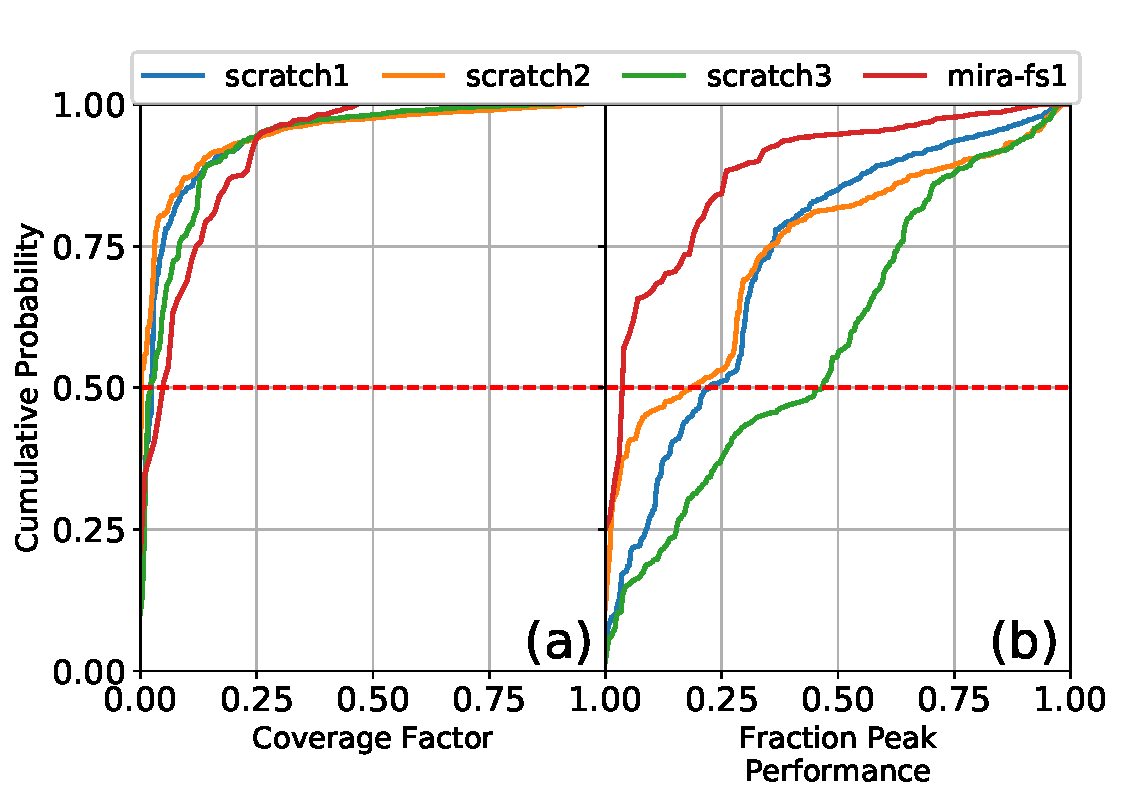
\includegraphics[width=\columnwidth]{figs/cdf-both.pdf}
	\caption{Cumulative distribution function of the coverage factor (a) and the
	performance relative to the maximum throughput observed across each file system
	(b).  The line demarcating 50\% probability corresponds to coverage factors of
	0.028, 0.004, 0.015, and 0.050 and peak performance fractions of 0.227, 0.185,
	0.467, and 0.040 on Edison scratch1-scratch3 and Mira, respectively.}
	\label{fig:cdfs}
\end{figure}

\begin{figure}[t]
	\centering
	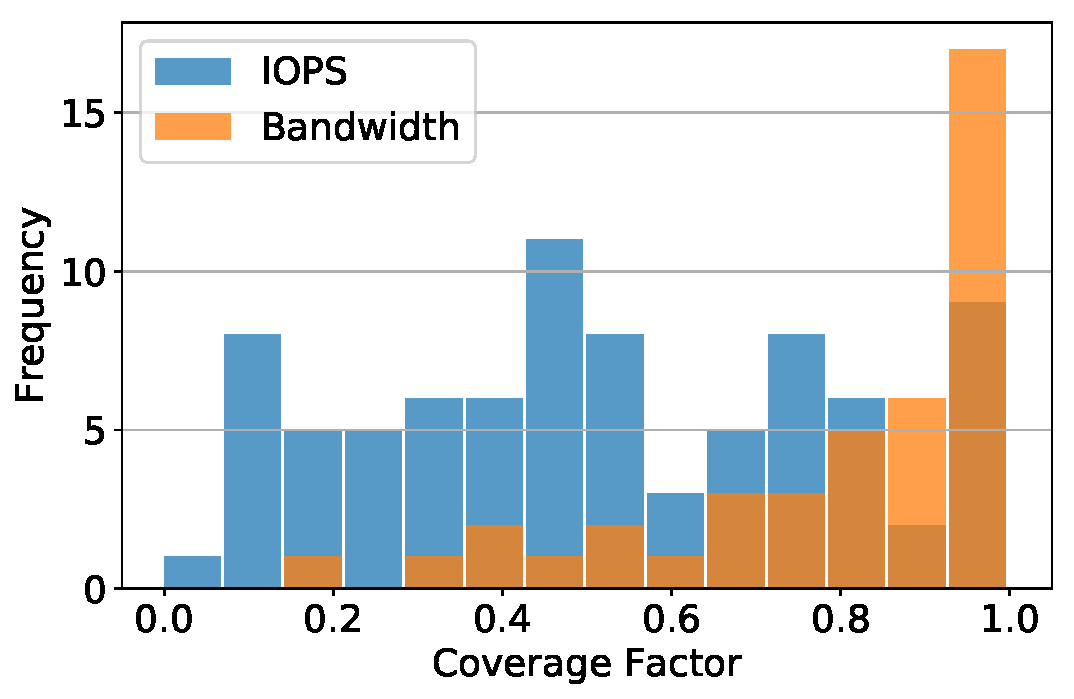
\includegraphics[width=\columnwidth]{figs/hist-cf-bw-and-ops.pdf}
	\caption{Distribution  of the coverage factor for both bandwidth ($\textit{CF}_{\textup{bandwidth}}$) and read/write operations ($\textit{CF}_{\textup{iops}}$) for Mira.
    }
	\label{fig:hist-cf-mira}
\end{figure}

To understand the relationship between IOP contention and performance degradation, we can also calculate the coverage factor of IOPS in addition to the coverage factor of bandwidth described in Equation \ref{eq:cf}.  If the relationship between performance and bandwidth is proportionately affected by IOPS-based contention, we would expect the coverage factor of IOPS to follow a similar distribution.  However, as shown in Figure \ref{fig:hist-cf-mira}, $\textit{CF}_{\textup{iops}}$ for Mira jobs are broadly distributed, whereas $\textit{CF}_{\textup{bandwidth}}$ shows a clear bias towards high values.  From this, we can conclude that many tests on Mira achieved high performance despite other I/O loads concurrently generating commensurate IOP loads.  None of the I/O motifs used here were designed to generate a significant number of IOPs though, so this may be simply an indication that the Mira file system can deliver reliable performance even under modest aggregate IOP loads coming from its applications.

%%%%%%%%%%%%%%%%%%%%%%%%%%%%%%%%%%%%%%%%%%%%%%%%%%%%%%%%%%%%%%%%%%%%%%%%%%%%%%%%
\subsection{Correlating Different Data Sources} \label{sec:results/correlating}
%%%%%%%%%%%%%%%%%%%%%%%%%%%%%%%%%%%%%%%%%%%%%%%%%%%%%%%%%%%%%%%%%%%%%%%%%%%%%%%%

Our choice to define our correlation parameter according to application performance and server-side bandwidth and IOPs was motivated by a broad body of literature and an intuitive assumption that competition for bandwidth and IOPs affect performance the most dramatically.  However, the TOKIO framework is generalized to draw data from any resource that can be indexed on a per-job or time series basis. As such, we can attempt to correlate a wide variety of measurements to job I/O performance to determine which measurements are likely culprits when looking for sources of poor I/O performance.

To this end, we calculated the Pearson correlation coefficient between each job's fraction of peak performance (as defined in Section \ref{sec:results/overview} ) with a wide range of metric collected on Edison and Mira, and the most interesting results are summarized in Figure \ref{fig:correlation-table}.  Although an exhaustive examination of all correlations is beyond the scope of this work, several key points can be gleaned by what these data do \emph{and do not} show.

\begin{figure}[t]
	\centering
	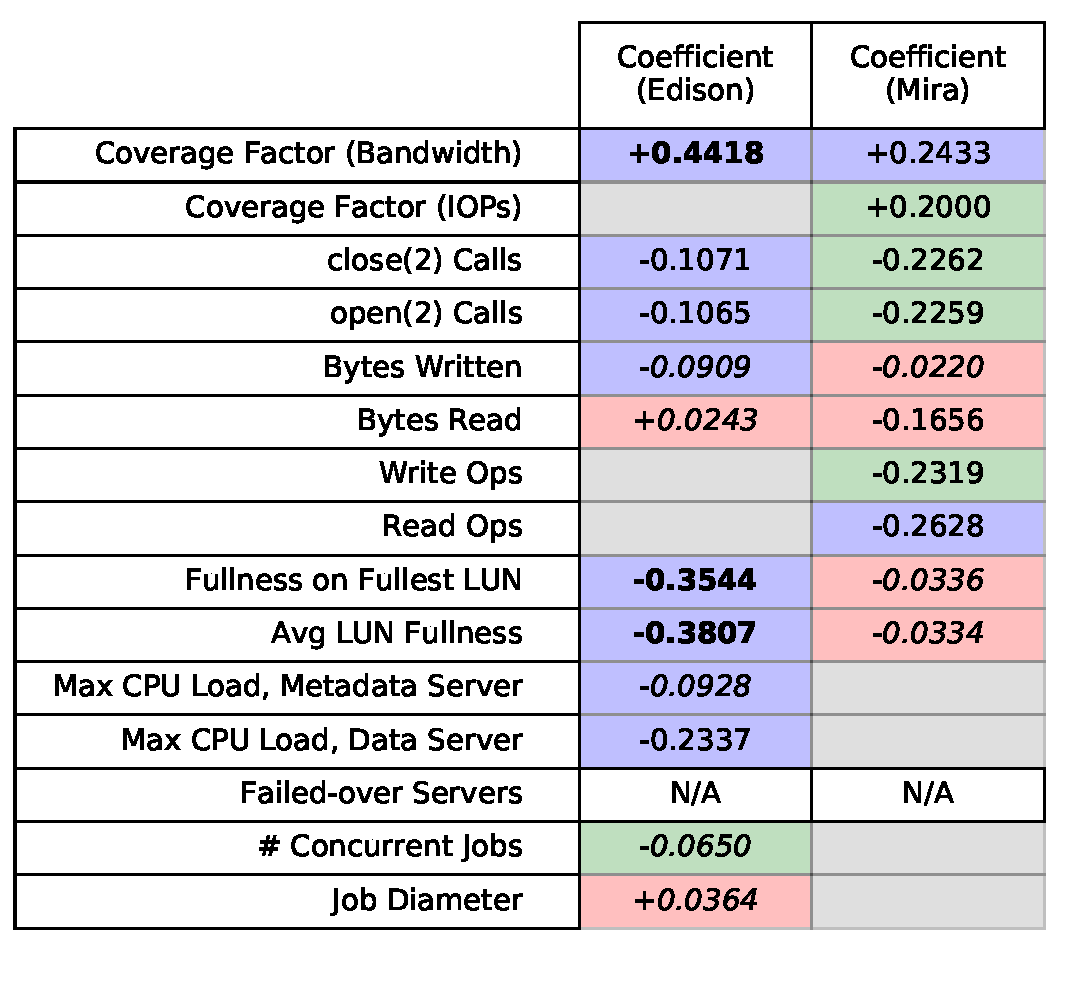
\includegraphics[width=\columnwidth]{figs/correlation_table.pdf}
	\caption{Correlation coefficients between fraction of peak performance measured for each I/O motif and a variety of server-side measurements and metrics.  Box color indicates confidence; correlations with p-values $< 0.01$ are blue; p-values $< 0.05$ are green, and p-values $>= 0.05$ are red (and signify lack of correlation).  Similarly, bolded values signify moderate correlation ($|r| > 0.30$), and italicized values signify weak correlation ($|r| < 0.10$).  Although the "\% Servers Failed Over" measurement were tracked on both Mira and Edison, no changes in the
    failover states of servers were ever observed over the course of this study.
    }
	\label{fig:correlation-table}
\end{figure}

\begin{itemize}

\item As assumed in the previous sections, the coverage factors correlate most strongly with performance on all file systems, indicating that contending for file system I/O is a moderate contributor to performance loss.  Mira's file system also demonstrated moderate sensitivity to contention for IOPs; unfortunately, Lustre IOPs were not collected for this study, so no comparison can be made to Edison.

\item Mira's performance correlates negatively with higher rates of \texttt{open(2)}/\texttt{close(2)} calls than Lustre.  Given
that Mira's file system encodes metadata in the same physical servers as data
blocks, this relationship is reasonable.  By comparison, Edison's file systems each have their own discrete metadata servers are specifically designed to decoupled bulk data transfer performance from metadata operations.

\item The fullness of each storage device (LUN on Mira and OST on Edison) has markedly different behavior between Edison and Mira.  While Mira's performance is uncorrelated with device capacity, Edison performance degrades as free space on OSTs is depleted.  This is a documented behavior of Lustre file systems.

\item Perhaps contrary to historic intuition, I/O performance shows no meaningful correlation with the number of other jobs running concurrently.  The lack of correlation with concurrent job count is consistent with our finding that I/O remains highly bursty; a large number of small jobs are highly unlikely to burst simultaneously, and each small job is not individually capable of impacting our tests' coverage factors.

\item Similarly, the job diameter (a measurement of how spread out a job is across the compute fabric) has no discernible correlation with I/O performance on Edison.  Given the fact that the low-diameter dragonfly topology of Edison is designed to reduce the performance impact of job topology, this is consistent with expectation.

\end{itemize}

In addition to the measurements and metrics presented in Figure \ref{fig:correlation-table}, the TOKIO framework collected a larger number of system-specific measurements that did not correlate significantly to performance.  However it is important to underscore the fact that this demonstration was not intended to be exhaustive, and the correlations and p-values for the Edison system are likely diminished by the fact that all three Edison file systems, each with unique users, workloads, and governance policies, were combined for this analysis.

%%%%%%%%%%%%%%%%%%%%%%%%%%%%%%%%%%%%%%%%%%%%%%%%%%%%%%%%%%%%%%%%%%%%%%%%%%%%%%%%
\subsection{Unified Measurements and Metrics Interface} \label{sec:results/umami}
%%%%%%%%%%%%%%%%%%%%%%%%%%%%%%%%%%%%%%%%%%%%%%%%%%%%%%%%%%%%%%%%%%%%%%%%%%%%%%%%

By establishing an understanding of the baseline distribution of performance for each I/O motif and file system in Sections \ref{sec:results/overview} and \ref{sec:results/combining} and identifying how different measurements and metrics correlate with performance in \ref{sec:results/correlating}, we now have a foundation from which we can describe

\begin{enumerate}
\item where on the spectrum of normalcy a specific job's I/O behavior fell relative to other jobs with a similar I/O motif, and
\item which measurements and metrics are the best places to start investigating abnormal conditions based on how they have historically correlated with performance
\end{enumerate}

To concisely visualize all of this information, we present the TOKIO Unified Measurements and Metrics Interface (UMAMI), shown in Figure \ref{fig:umami-scratch2-hacc-write}, with the goal of enabling end-users to quickly see how their application's performance compares
to similar I/O workloads in the past.  TOKIO-UMAMI presents historic measurements from the components monitored by TOKIO, composing what we refer to as the \emph{I/O subsystem climate}, and summarizes each metric's distribution in a box plot to the right of each metric's time series plot.  These time series plots terminate with the measurements taken for the job in question, describing the \emph{I/O subsystem weather} at the time that job ran.  By overlaying this weather on the climate box plots in the form of dashed lines, TOKIO-UMAMI provides a quick visualization of how each metric's weather compared to the statistical distribution of past weather conditions.  This conceptualization of a file system's weather with its overall climate, a user can differentiate between a long-term performance problem (as would occur if the application I/O is not optimized for the underlying file system) and a statistically rare event analogous to an extreme weather event.

The specific UMAMI example shown in Figure \ref{fig:umami-scratch2-hacc-write} represents a HACC write test which took place on March 3.  This particular job showed abnormally low performance as evidenced by the "Job performance (GiB/sec)" measurement and its value relative to the previous six instances of this type of job.  This abnormally poor job performance was accompanied by an unusually low coverage factor and high metadata load, and these unfavorable conditions (which fell into the bottom-most quartile of past measurements) are highlighted as red dashed lines in the box plots.  The metrics corresponding to blue dashed lines fell into the uppermost quartile for this problematic job, but as discussed in Section \ref{sec:results/correlating}, have no history of correlation with performance.  Thus, we can quickly attribute the poor performance of this HACC job to an I/O extrinsic to this HACC job which was competing for both bandwidth on the data servers and metadata resources on the metadata server.

\begin{figure}[t]
	\centering
	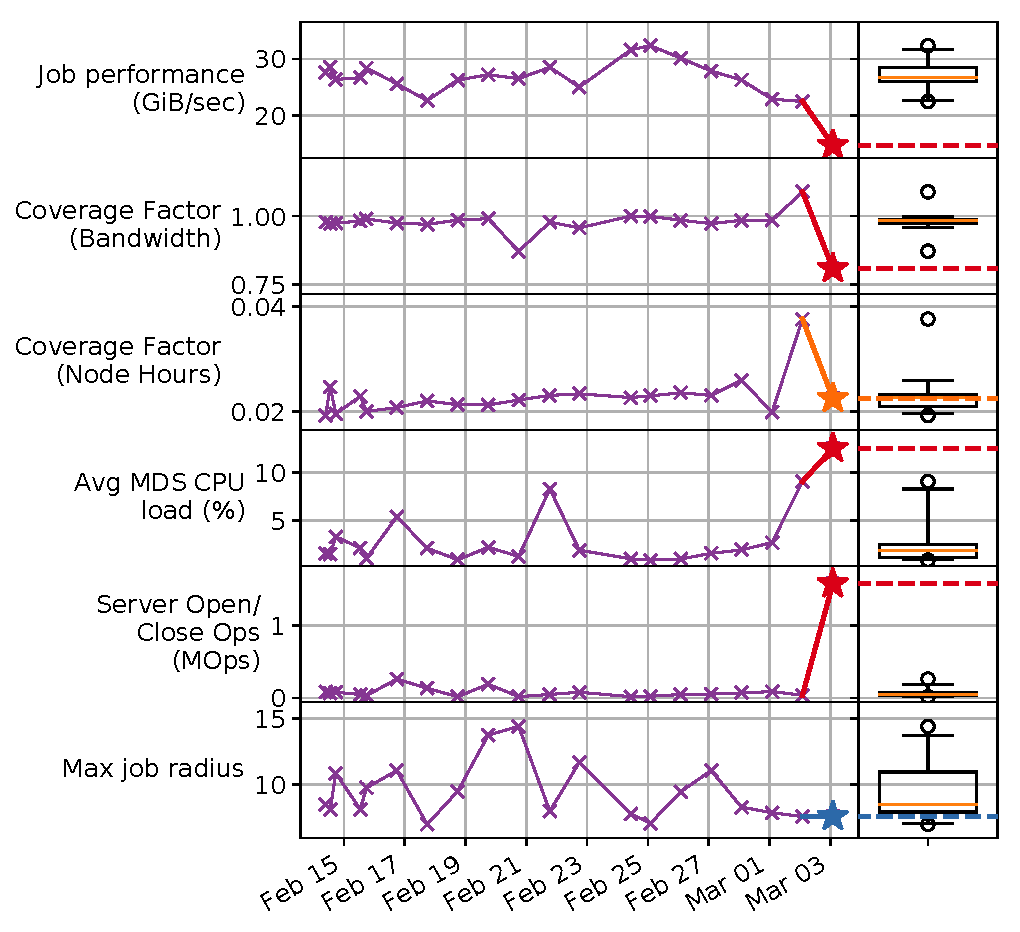
\includegraphics[width=1.0\columnwidth]{figs/umami-scratch2-hacc-write.pdf}
	\caption{TOKIO-UMAMI demonstrating the \emph{file system climate} of HACC write workloads
	on the Edison scratch2 file system compared to a most recent run, which showed
    highly unusual \emph{file system weather}.}
	\label{fig:umami-scratch2-hacc-write}
\end{figure}

Similarly, Figure \ref{fig:umami-mira-fs1-vpic-write} represents a VPIC write workload that showed poor performance on Mira.  However, its coverage factor is within normal parameters (denoted by an orange line in the box plot, indicating its value is in the second quartile) indicating a general lack of bandwidth contention.  Although the IOPS coverage factor is also abnormally low, previous conditions have been worse despite a lack of dramatic performance loss.  The only metric that shows an uncommonly undesirable value is the number of \emph{readdir(3)} operations handled by the file system, which is indicative of an expansive file system traversal and was demonstrated to correlate moderately with performance in Figure \ref{fig:correlation-table}.

\begin{figure}[t]
	\centering
	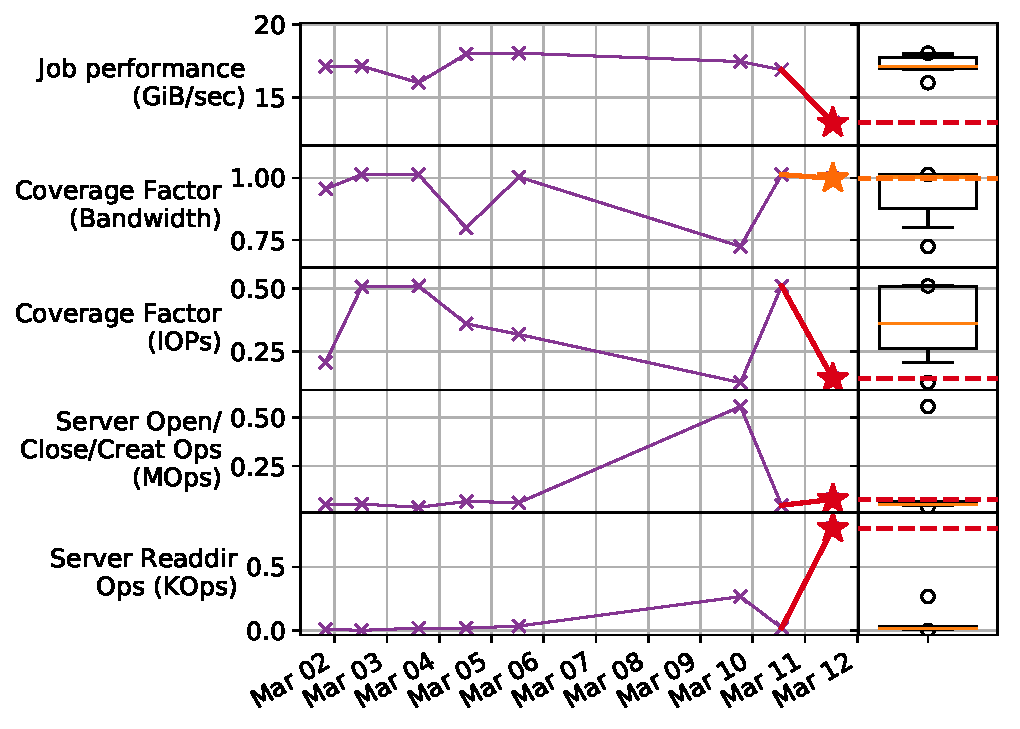
\includegraphics[width=1.0\columnwidth]{figs/umami-mira-fs1-vpic-write.pdf}
	\caption{TOKIO-UMAMI demonstrating the \emph{file system climate} of VPIC-IO read workloads
	on Mira compared to a most recent run, which showed
    highly unusual \emph{file system weather}.}
	\label{fig:umami-mira-fs1-vpic-write}
\end{figure}

%%%%%%%%%%%% this is as far as I've gotten on my most recent pass
\hrulefill

%%%%%%%%%%%%%%%%%%%%%%%%%%%%%%%%%%%%%%%%%%%%%%%%%%%%%%%%%%%%%%%%%%%%%%%%%%%%%%%%
\subsection{Discussion} \label{sec:results/discussion}
%%%%%%%%%%%%%%%%%%%%%%%%%%%%%%%%%%%%%%%%%%%%%%%%%%%%%%%%%%%%%%%%%%%%%%%%%%%%%%%%

This section will discuss \emph{why} we saw the behavior that we did by
aligning and correlating data sources, then make broader conclusions about the
differences
between Mira and Edison results.


With this framework, we then deep-dive into several specific cases of
performance degradation identified by the TOKIO dashboard.  For example,
(\ref{fig:umami-scratch2-hacc-write}) shows a particular date (March 4) on
which performance was abnormally low while both the coverage factor and metadata
open/close rates were abnormal.

We also know that VPIC-IO behaves very differently on Mira vs. Edison, and this
might make a good deep dive.  Similarly, understanding HACC's long tail would
be great.

Once we have shown that we understand several different sources of performance
loss, we can then establish a taxonomy and enumerate how often bad I/O
performance can be attributed to each of the different causes we categorized so
that we can offer one or two specifically common sources of interference.  For
example,

\begin{itemize}
\item Sometimes metadata operations are slow (e.g., file-per-process I/O)
    \begin{itemize}
    \item Show Darshan logs showing high metadata time
    \item Show LMT MDT logs showing high background metadata or CPU rate
    \item Show GPFS NSD metadata loads?  Can we do this?
    \end{itemize}
\item Sometimes hardware goes bad
    \begin{itemize}
    \item Show Darshan logs showing bad performance at the POSIX layer (i.e., not the
    application's fault)
    \item Show Lustre OSTs that stall out
    \item Show slow Lustre OSTs due to failover/oversubscription (a la Darshan 3 paper)
    \item Show poorly performing GPFS NSDs
    \end{itemize}
\item Sometimes there is interference from other applications
    \begin{itemize}
    \item Show Darshan logs showing bad performance at the POSIX layer (i.e., not the
    application's fault)
    \item Show jobs with and without background LMT load
    \item Show jobs with and without background mmpmon load
    \end{itemize}
\item Sometimes tuning strategies differ across platforms
    \begin{itemize}
    \item contrast which benchmark performs best on each platform
    \item dig into why
%   \item See example of how we might show this in Figure~\ref{fig:example-bar-var}
    \end{itemize}
\end{itemize}

If we have enough data to make a statistically significant statement, we should
aim to discuss how susceptible different file systems are to these bad I/O
performance root causes to stir up controversy (GPFS is better/worse than
Lustre when facing problem X).  If we do this, we can also propose strategies
to work around these common bottlenecks.  For example, can holistic I/O
monitoring provide a feedback loop for coscheduling?  These would be stretch
statements.

In addition, we can point out that the dashboard is most useful when an historic
record of similar jobs executions is already known \emph{a priori}, Liu et al~\cite{Liu2016}
has demonstrated that it is possible to combine resource manager logs alongside
server-side I/O logs to identify a series of I/O bursts with specific jobs,
users, and applications.  Future work may be to incorporate this I/O pattern
identification algorithm with the TOKIO dashboard to automatically build an
historic record for any arbitrary job.

It may also be worth saying that the TOKIO dashboard can display an historic
record for any grouping of I/O patterns.  Although groupings were established
around specific applications based on Darshan logs, it is equally useful to
use groupings built around similar periods of server-side traffic.  For example,
it is possible to identify collections of applications that, when run together,
produce abnormally poor server-side performance or, conversely, surprisingly
good performance.  From this would arise an opportunity to inform scheduling
to optimize for or avoid I/O contention between two frequently conflicting
applications.


\section{Related work} \label{sec:related}

\assign{Phil} \todo{include SIOX} Let's cite Xiaosong Ma's work in server-side
monitoring \cite{Liu2016}; her work uses server-side logs to make scheduling
recommendations based on a knowledgebase of applications and their historic
I/O requirements.  This work can improve the predictive ability of such systems
by replacing the black-box weighting parameter, $w_{i}$, with a function that
accurately captures the effects of different external interference sources for
an application.

Matthieu showed how to minimize I/O jitter~\cite{Dorier2012} (but I haven't read
this paper yet...).  More recently, Yildiz et al~\cite{Yildiz2016} performed
a systematic exploration of points of contention on an idealized system and
exposed the sensitivity of 10 GbE to various forms of interference.

Lofstead et al wrote a paper on managing I/O variability in production~
\cite{Lofstead2010} which characterized \emph{internal interference} and
\emph{external interference} using purely client-side metrics.  They defined an
\emph{imbalance factor}, the ratio of the slowest to fastest write times, as a
means to infer the external interference, but we can precisely quantify it here
with server-side metrics.

Andrew Uselton's work on understanding I/O performance in terms of ensembles of
bursts might be relevant\cite{Uselton2010}, but his method requires heavyweight
I/O tracing to determine the statistical distribution of I/O bursts during an
application execution and, as such, as better suited to characterizing the
behavior of a specific file system as a one-time activity.

A long time ago, David Skinner and Bill Kramer wrote a paper that characterized
sources of performance variation~\cite{Skinner2005}, but it didn't really talk
about I/O in a very meaningful way.

More recently Xie et al also characterized I/O problems at Oak
Ridge\cite{Xie2012} using IOR and quantified the effects of stripe counts,
straggling writers, and shared-file I/O to target areas where middleware can
optimize I/O for applications.

Is any of the BeeGFS stuff (dynamically provisioning file systems) relevant to
interference isolation?

\section{Conclusions} \label{sec:conclusions}

\todo{It would be great if there were some tangible artifacts from this work.
Possible examples:}
\begin{itemize}
\item open repo for benchmark configs and cron jobs so others can replicate
performance regression testing
\item anonymized data collected in study
\item new data collection tools (LMT monitoring, Lustre failover monitoring,
mmpmon monitoring, etc.)
\end{itemize}

\section{TEMPORARY: TECHNICAL TASKS}

Assumption: assignments here and in preceding text are tentative, and really
just guess at someone who can keep tabs on that activity.  Can re-assign,
delegate, pull in more people, etc.

\begin{itemize}
    \item \textcolor{red}{ALL}: Begin analyzing TOKIO-ABC benchmark results and
    and think about how we want to correlate this with GPFS/Lustre monitoring
    data. Are there specific jobs or timeframes that we want to zoom in on
    to better understand anomalous behavior? Are there I/O trends that we
    can observe on specific systems or even across systems that would be
    interesting to the reader? This is where we want to showcase the utility
    of this framework, so we will need to find something interesting to demonstrate
    here to convince the reader. 

    \item \textcolor{red}{ALL}: begin filling in paper intro, background,
    methodology, system/benchmark descriptions, results, etc.

    \item \textcolor{red}{SHANE}: round up MMPMON data for a 2-week period
    of TOKIO-ABC runs on Mira.

    \item \textcolor{red}{GLENN}: round up LMT data for a 2-week period of
    TOKIO-ABC runs on Edison.

    \item \textcolor{red}{WILLIAM}: look at MMPMON data to determine how
    IOMiner can be extended to analyze GPFS data. 
\end{itemize}

Timeline:
\begin{itemize}
    \item \textcolor{red}{SC abstracts due March 20, 2017}
    \item \textcolor{red}{SC full submissions due March 27, 2017}
    \item Time to get moving!
\end{itemize}

\bibliographystyle{IEEEtran}
\bibliography{REFERENCES}

\appendix

\section{Artifact Description}

Consider adding material here per guidance at
\url{http://sc17.supercomputing.org/2017/02/07/submitting-a-technical-paper-to-sc17-participate-in-the-sc17-reproducibility-initiative/}.

\end{document}
